\documentclass[10 pt, twocolumn]{article}

\usepackage[utf8]{inputenc}
\usepackage[T1]{fontenc}
\usepackage{caption}
\usepackage{graphicx}
\usepackage{xcolor}
\usepackage{interval}
\usepackage{listingsutf8}
\usepackage{hyperref}
\usepackage{siunitx}
\usepackage{algorithm2e}
\usepackage{rotating}
\usepackage{adjustbox}
\usepackage{booktabs}
\usepackage{pgfplots}
\usepackage{tikz}
\usepackage{footmisc}
\usepackage{amsfonts}
\usepackage[backend=biber,style=numeric]{biblatex}
\usepackage[
  left=1.50cm,
  right=1.50cm,
  top=2.00cm,
  bottom=2.00cm
]{geometry}

\pgfplotsset{compat=1.15}

\sisetup{load-configurations=abbreviations, binary-units=true}
\intervalconfig {
    soft open fences ,
    separator symbol =; ,
}

\lstdefinelanguage{JavaScript}{
  keywords={break, case, catch, continue, debugger, default, delete, do, else, finally, for, function, if, in, instanceof, new, return, switch, this, throw, try, typeof, var, void, while, with},
  morecomment=[l]{//},
  morecomment=[s]{/*}{*/},
  morestring=[b]',
  morestring=[b]",
  sensitive=true
}

\lstdefinelanguage{Protobuf}{
  keywords={message, string, uint32, int32},
  morecomment=[l]{//},
  morecomment=[s]{/*}{*/},
  morestring=[b]',
  morestring=[b]",
  sensitive=true
}

\lstset{
    language=C,
    keywordstyle={\bfseries},
    basicstyle=\footnotesize,
    literate={->}{$\rightarrow{}$}{1} {<-}{$\leftarrow{}$}{1},
    stringstyle=\color{purple},
    keepspaces=true,
    captionpos=b,
    inputencoding=utf8,
    escapeinside={\%*}{*)}
}

\renewcommand\AlCapSty{\text}
\SetAlCapNameFnt{\footnotesize}
\SetAlCapFnt{\footnotesize}
\SetAlgoCaptionSeparator{.}
\DeclareCaptionLabelFormat{nospace}{#1 #2}
\captionsetup[table]{labelformat=nospace,labelfont=rm,name=Table,labelsep=period}

\newcommand{\pcode}[1]{
    \lstinline[basicstyle=\itshape,keywordstyle={}]{#1}
}

\newcommand*{\lstnumberautorefname}{line}

\newcommand{\icode}[1]{\lstinline{#1}}

\newcommand{\name}[1] {\emph{#1}}

\newcolumntype{R}[2]{%
    >{\adjustbox{angle=#1,lap=\width-(#2/2)}\bgroup}%
    l%
    <{\egroup}%
}
\newcommand*\rot{\multicolumn{1}{R{90}{1em}}}

\newcommand{\fig}[3]{
  \begin{figure}[h]
    \begin{center}
        \includegraphics[width=8cm,keepaspectratio]{#1}
        \caption{#3}
        \label{fig:#2}
    \end{center}
  \end{figure}
}

\usepackage[most]{tcolorbox}
\newcounter{example}
\usepackage{xparse}
\usepackage{lipsum}

\def\exampletext{Example} % If English
\NewDocumentEnvironment{example}{ O{} }
{
\colorlet{colexam}{red!55!black} % Global example color
\newtcolorbox[use counter=example]{examplebox}{%
    % Example Frame Start
    empty,% Empty previously set parameters
    title={#1},% use \thetcbcounter to access the example counter text
    % Attaching a box requires an overlay
    attach boxed title to top left,
       % Ensures proper line breaking in longer titles
       minipage boxed title,
    % (boxed title style requires an overlay)
    boxed title style={empty,size=minimal,toprule=0pt,top=4pt,left=3mm,overlay={}},
    coltitle=colexam,fonttitle=\bfseries,
    before=\par\medskip\noindent,parbox=false,boxsep=0pt,left=3mm,right=0mm,top=2pt,breakable,pad at break=0mm,
       before upper=\csname @totalleftmargin\endcsname0pt, % Use instead of parbox=true. This ensures parskip is inherited by box.
    % Handles box when it exists on one page only
    overlay unbroken={\draw[colexam,line width=.5pt] ([xshift=-0pt]title.north west) -- ([xshift=-0pt]frame.south west); },
    % Handles multipage box: first page
    overlay first={\draw[colexam,line width=.5pt] ([xshift=-0pt]title.north west) -- ([xshift=-0pt]frame.south west); },
    % Handles multipage box: middle page
    overlay middle={\draw[colexam,line width=.5pt] ([xshift=-0pt]frame.north west) -- ([xshift=-0pt]frame.south west); },
    % Handles multipage box: last page
    overlay last={\draw[colexam,line width=.5pt] ([xshift=-0pt]frame.north west) -- ([xshift=-0pt]frame.south west); },%
    }
\begin{examplebox}}
{\end{examplebox}\endlist}

\newcommand*\circled[1]{\tikz[baseline=(char.base)]{
            \node[shape=circle,draw,inner sep=1pt] (char) {#1};}}

\usepackage{tikz}

\newcommand{\smiley}{\tikz[baseline=-0.75ex,black]{
    \draw circle (2mm);
\node[fill,circle,inner sep=0.5pt] (left eye) at (135:0.8mm) {};
\node[fill,circle,inner sep=0.5pt] (right eye) at (45:0.8mm) {};
\draw (-145:0.9mm) arc (-120:-60:1.5mm);
    }
}

\newcommand{\frownie}{\tikz[baseline=-0.75ex,black]{
    \draw circle (2mm);
\node[fill,circle,inner sep=0.5pt] (left eye) at (135:0.8mm) {};
\node[fill,circle,inner sep=0.5pt] (right eye) at (45:0.8mm) {};
\draw (-145:0.9mm) arc (120:60:1.5mm);
    }
}

\newcommand{\neutranie}{\tikz[baseline=-0.75ex,black]{
    \draw circle (2mm);
\node[fill,circle,inner sep=0.5pt] (left eye) at (135:0.8mm) {};
\node[fill,circle,inner sep=0.5pt] (right eye) at (45:0.8mm) {};
\draw (-135:0.9mm) -- (-45:0.9mm);
    }
}


\addbibresource{root.bib}

\title{Machine Learning to the rescue}

\author{Jan Macháček}

\newcommand{\joel}[1]{\\ \emph{Joel: #1}}
\newcommand{\pc}[1]{\lstinline[basicstyle=\small,columns=fixed]|#1|}
\usetikzlibrary{positioning}

\tikzset{
    table/.style={
           rectangle,
           draw=black, very thick,
           minimum height=2em,
           inner sep=2pt,
           text centered,
           },
}

\begin{document}

\twocolumn[
  \begin{@twocolumnfalse}
    \maketitle
    \begin{abstract}
      Machine learning to the rescue!... the first question is ``to the rescue of what?''; immediately followed by ``when is it indeed rescued?''. The answers to these questions are crucial; luckily, the software engineering process is quite used to asking and answering these questions. Careful project analysis and inception, followed by continous integration and continous deployment in development (supported by adequate tests); all overseen by systematic project governance leads to successful software projects. This paper's proposition is that machine learning projects that are to apply established machine learning approaches and algorithms are no different than any other software project; and they must follow all practices of software engineering. 
    \end{abstract}
  \end{@twocolumnfalse}
]

\section{Software engineering}
...

The Joel test\cite{joeltest} is a product of one man's biased, ad-hoc, informal, ... view of what makes successful software projects. Annoyingly, high scores on the Joel test correlate with successfully delivered software projects. Spolsky acknowledges that it's possible for a small team of cowboys to deliver amazing software with score of 0, as much as it is possible for a team that scores 12 to be the software equivalent of the Titanic. Nevertheless, high scores on the test correlate with good practices and discipline, which usually leads to good software.

This paper's proposition is that ``business'' projects that use machine learning are no different than any other software project; and that all practices of software engineering have to be applied to the machine learning subsystems. Specifically, that the 12 points on the Joel test are just as applicable, but with additional 12 points. 

\begin{enumerate}
  \item Version control for the ML models and data sets used to train them
        \joel{Do you use source control?}
  \item Single-step / automated data selection, model training, evaluation, and deployment
        \joel{Can you make a build in one step?}
  \item [At least] daily training and deployment process
        \joel{Do you make daily builds?}
  \item The results of the BI queries that humans process define what ML should solve
        \joel{Do you have a bug database?}
  \item Versioned, testable; continuously tested and sanity-checked BI
        \joel{Do you fix bugs before writing new code?}
  \item BI that allows any query to be answered in under 10 minutes
        \joel{Do you have a spec?}
Do you have an up-to-date schedule?
Do programmers have quiet working conditions?
Do you use the best tools money can buy?
Do you have testers?
Do new candidates write code during their interview?
Do you do hallway usability testing?
  \item Versioned, testable; continuously tested and sanity-checked analytics (BI)  
  \item Monitoring on the BI environment to identify queries that use normalised data
  \item The results of the BI queries that humans process define what ML should solve
  \item Ingestion components decoupled from the rest of the system
  \item Versioned, testable; continuously tested and sanity-checked data sets 
  \label{txt:ml-code}\item Pre-computed ``return constant'' model
  \item Versioned, testable; continuously tested and sanity-checked model storage with training and validation data set references
  \item Model deployer and ``debugger''
\end{enumerate}

\begin{enumerate}
  \item Versioned, testable; continuously tested and sanity-checked analytics (BI)  
  \item Any BI query can be answered under 10 minutes
  \item Monitoring on the BI environment to identify queries that use normalised data
  \item The results of the BI queries that humans process define what ML should solve
  \item Ingestion components decoupled from the rest of the system
  \item Versioned, testable; continuously tested and sanity-checked data sets 
  \label{txt:ml-code}\item Pre-computed ``return constant'' model
  \item Versioned, testable; continuously tested and sanity-checked model storage with training and validation data set references
  \item Model deployer and ``debugger''
\end{enumerate}

But where is the ML that builds the model? That's the code that the engineering teams need to build to replace \autoref{txt:ml-code}. 

Once the first four steps are known, the engineering teams can implement the remaining steps of the pipeline. If the system that is to take advantage of ML is event-based, the event delivery mechanism provides the decoupling, resulting in architecture shown in \autoref{fig:pipeline-es}.

\fig{pipeline-es.png}{pipeline-es}{ML pipeline in event-based system}

If the front-end system is not event-sourced, the ingestion must be decoupled using a read-only replica of the live data. Notice in \autoref{fig:pipeline-nes} the flow of the data: the data is pushed into the read-only replica in the first step to allow the front-end system to control the load on its data store; from the read-only replica, the data is pulled into the ML data store. 

\fig{pipeline-nes.png}{pipeline-nes}{ML pipeline in non event-based system}

Regardless of the approach used (or even if a hybrid approach is deployed), the entire system has to be aware of any back-pressure.

The ML team maintains the tooling for the pipeline, consults on the best models, researches, ...; but the product teams (that ultimately work on the service that \emph{uses} the model) have the first dibs on implementing the model. Successful implementation of this strategy means that anyone can implement a new model (even if only to just see what will happen!), train it, debug it, and deploy it all within a single day. All the mechanics of data ingestion, storage, versioning; runtime of training a model, evaluation, storage, versioning; debugging and deploying; and the usage is all implemented. 

In this sense, the machine learning code is just like any other ordinary code; it is subject to all the high engineering standards and safeguards.

\section{Implementation choices}
Attach technologies to the blocks in \autoref{fig:pipeline-es} and \autoref{fig:pipeline-nes}. Show on practical example, attempt to pull out reusable blocks and show examples of good and bad code. Think the recent ML experiments; demonstrating just how much time the initial research and experiments take. Reinventing the experimental wheel must be avoided--the ML team should curate the bootstrapping environment, making it available ``on demand'' for other teams. The work on the ML core code can only successfully happen when all other pieces are in place. 

\subsection{Initial research}
The practical application of the ``ML enablement process'' aimed to deliver failure predictions and automatic error recovery based in an event-based architecture system. The system already published seemingly too many events, but the detail in the events were very useful in building the data sets for the ML project. The first step the team needed to take was to build traditional business intelligence database--the goal was to find out whether our human knowledge and experience allowed us to find meaningful information in the data.

The system's journal (Apache Kafka\cite{kafka}) is configured with 7 days' message retention policy; at the very start of the work, the team was able to download events for the last 7 days. This was approximately \SI{60}{\gibi\byte} of uncompressed Protocol Buffers\cite{protobuf} binary messages. Because of the compactness of the binary wire representation of the Protocol Buffers messages, this translated to \SI{60}{\gibi\byte} of a RDBMS (MySQL\cite{mysql}) storage requirements. The loader program performed batch JDBC inserts into the MySQL tables. The events in the \pcode{HttpRequest} and \pcode{HttpResponse} topics were imported to the matching tables, the events in the \pcode{ServiceStateChanged}, \pcode{ServiceStateUnchanged}, \pcode{ServiceAdded}, and \pcode{ServiceRemoved} were pre-processed and inserted into the \pcode{Service} table. The tables are not even in the 1\textsuperscript{st} normal form; there is only the primary key, but there are no foreign key constraints; during the batch import, there are no indexes. 

\begin{figure}
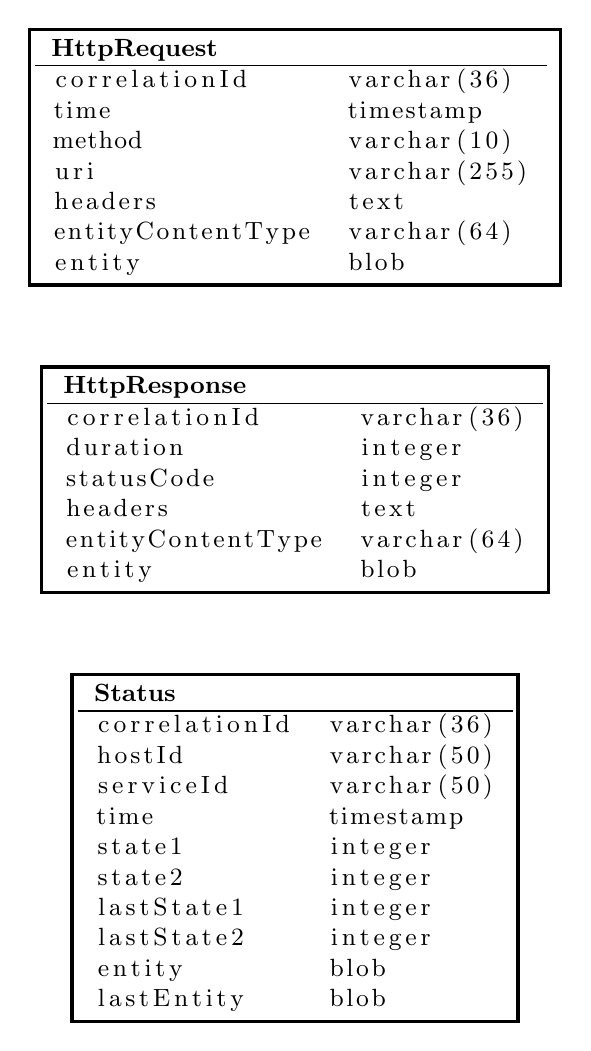
\begin{tikzpicture}
  \tikzstyle{every node}=[font=\small] 
  \node[table, align=left] (HttpRequest)
  {
    \begin{tabular}{ll}
      \textbf{HttpRequest} \\\hline
      \pc{correlationId}     & \pc{varchar(36)} \\
      \pc{time}              & \pc{timestamp} \\
      \pc{method}            & \pc{varchar(10)} \\
      \pc{uri}               & \pc{varchar(255)} \\
      \pc{headers}           & \pc{text} \\
      \pc{entityContentType} & \pc{varchar(64)} \\
      \pc{entity}            & \pc{blob} \\
    \end{tabular}
  };

  \node[table
       , below=1cm of HttpRequest
       ] (HttpResponse)
  {
    \begin{tabular}{ll}
      \textbf{HttpResponse} \\\hline
      \pc{correlationId}     & \pc{varchar(36)} \\
      \pc{duration}          & \pc{integer} \\
      \pc{statusCode}        & \pc{integer} \\
      \pc{headers}           & \pc{text} \\
      \pc{entityContentType} & \pc{varchar(64)} \\
      \pc{entity}            & \pc{blob} \\
    \end{tabular}
  };

  \node[table
       , below=1cm of HttpResponse
       ] (Status)
  {
    \begin{tabular}{ll}
      \textbf{Status} \\\hline
      \pc{correlationId}     & \pc{varchar(36)} \\
      \pc{hostId}            & \pc{varchar(50)} \\
      \pc{serviceId}         & \pc{varchar(50)} \\
      \pc{time}              & \pc{timestamp} \\
      \pc{state1}            & \pc{integer} \\
      \pc{state2}            & \pc{integer} \\
      \pc{lastState1}        & \pc{integer} \\
      \pc{lastState2}        & \pc{integer} \\
      \pc{entity}            & \pc{blob} \\
      \pc{lastEntity}        & \pc{blob} \\
    \end{tabular}
  };

  \end{tikzpicture}
  \label{fig:erd}
  \caption{Database schema}
\end{figure}

The first seven days' worth of data import ended up as \numprint{5103397} rows in \pcode{HttpRequest}, \numprint{5103397} rows in \pcode{HttpResponse}\footnote{The same number of rows in the \pcode{HttpRequest} and \pcode{HttpResponse} is a very good sanity-check!}, and \numprint{54566575} rows in \pcode{Service}. This imported database was the starting point for the human analysis code. ``How many \pcode{statusCode != 200} in \pcode{HttpResponse} are there?''--(\numprint{72796}); ``what is the average response duration?''--(\SI{4.0759}{\milli\second}); ``what is the average response duration for successful responses''--(\SI{4.9862}{\milli\second}), and so on. In order to answer these questions, the database needed a few indexes: remember, ``any ad-hoc analytics query needs to be answerable within 10 minutes.'' The \pcode{db.m4.4xlarge} instance was completely sufficient for the first 7 days' worth of data; even for the first 70 days' worth of data. It delivered just over \SI{150}{\mebi\byte\per\second} in read and write throughput, and with only a few users running queries, its CPU usage never got above 50 \%; it was allocated \SI{5}{\tebi\byte} of SSD storage. 

The first valuable answer came from the analysis of the frequency of different errors by joining \pcode{request} and \pcode{resonse} on \pcode{correlationId} where \pcode{statusCode != 200}, grouping and counting by \pcode{response.entity}. The top 3 errors turned out to be fairly simple to fix, and the fixes resolved 90 \% of all observed errors. Beyond the top 3, the errors had no trivial cause and no trivial fix; the team suspected that the errors were cause by a combination of parameters passed in the requests, the previous state of the device doing the work, the network conditions, ...; something that could not be trivially reproduced nor fixed. Interestingly, the 3 least frequent errors did turn out to have trivial fixes: in the sense that there was no fix, but better failure reporting in low or missing resource conditions, misconfiguration, etc.

These were great first results. The next valuable feature was to predict a failure before it actually happened, which would reduce the pressure \& stress in the operations team. 

uilding time series of requests, responses, and status changes. The tool was simple SQL \pcode{create table ... from select ... inner join}; the sequence of events ended up as \numprint{50182398} rows, describing \numprint{545357} sequences\footnote{Sanity-check: there are periodic health-checks for every service contributing nearly 80 \% of the HTTP requests and responses, and a typical sequence is made up of a single request and response, and multiple (usually $> 10$) service changed rows; there cannot be more sequences than requests and responses. The \numprint{545357} number of sequences is therefore a sane number of sequences, given the sizes of the tables}. The data had sequences such as $(req_1, res_1) \rightarrow \mathcal{I}dle, (req_2, res_2) \rightarrow \mathcal{B}usy, \ldots, (req_n, res_n) \rightarrow \mathcal{E}rror$, or even $(req_1, res_1) \rightarrow \mathcal{I}dle, (req_2, res_2) \rightarrow \mathcal{B}usy\text{ (without further requests) } \mathcal{E}rror$. This work implements the first part of the overall diagram (viz \autoref{fig:pipeline-bi}), and was able to satisfy (TODO) X, Y, and Z items on the ML readiness test.

\fig{pipeline-bi.png}{pipeline-bi}{Data collection and BI}

Nevertheless, this initial analysis was sufficient to build data sets for failure prediction.  the team deployed code more sophisticated than \pcode{select from ... group by ... having ...}.

\subsection{Buy vs. build (AWS services vs. custom code)}


\subsection{Testing}
Detect
\begin{itemize}
  \item unstable data (outliers, bad labels, etc.)
  \item underfitting (too little data)
  \item overfitting (too little data; model is a memoized map of input -> output)
  \item unpredictable future (with new data, is the model still stable?)
\end{itemize}

Seam testing: treat ML models as ``legacy black boxes'', but evaluate. Use cross-validation (split training and evaluation data sets). Measure and record:

\begin{itemize}
  \item precision--$TP / all predictions$ 
  \item recall--$TP / TP + FN$ 
  \item time taken to train
  \item model size
\end{itemize}

Use time-boxed computation to re-evaluate the performance of all previous models against the current validation data set.

Treat the output of the ML box as if it were a scientific experiment: what is the probability that the (good) results happened through chance rather than good performance of the classifier. Statistical tests on the output and the input data.

\section{Compromises}
How to manage the growing data sizes and time to train the models; particularly with complex models that need a lot of computation to train? Where to keep the old data and old models? Is there ever value in digging out models and data that are 10 versions old?

\printbibliography

\end{document}
